\section{Models}
% A description of the model(s) that you are evaluating/exploring. We are expecting a thorough
% exploration of at least 3+ family of models1, even if you don’t ultimately use those models. We are looking for:
% – How you are applying these models. You don’t need to reiterate what the models are and how they work. Instead, we’re looking for a description of the choices you are making to apply the model to this task: e.g., what features from the “Data” section are you using for each model? What adjustments (if any) did you need to make?

The setup of our training is similar for all models:
% Make a bullet point list
\begin{itemize}
    \item We used the cleaned and encoded data as described in \ref{sec:exploration}.
    \item We split the data into training, validation and test sets using a 60/20/20 split using \href{https://scikit-learn.org/stable/modules/generated/sklearn.model_selection.train_test_split.html}{train\_test\_split} from sklearn. We used a consistent random seed of 42 to ensure reproducibility.
    \item We used stratified sampling to ensure that the distribution of classes is similar in both sets.
    \item We used the same evaluation metrics for all models: accuracy, precision, recall, and F1-score.
    \item We used \href{https://rasbt.github.io/mlxtend/user_guide/evaluate/bias_variance_decomp/}{bias\_variance\_decomp} from mlxtend to calculate the bias and variance of our models.
    \item We used \href{https://scikit-learn.org/stable/modules/generated/sklearn.metrics.classification_report.html}{classification\_report} from sklearn to generate the classification report for our models.
\end{itemize}

\subsection{Multi Layer Perceptron (MLP)}

We started with training a \ref{https://scikit-learn.org/stable/modules/generated/sklearn.neural_network.MLPClassifier.html}{MLPClassifier}
on the cleaned and encoded data as described in \ref{sec:exploration} using the default parameters by
sklearn.
The default configuration is as follows:\\
Hidden layer: 1 layer, 100 hidden units\\
Activation: ReLu\\
We achieved an 90\% validation accuracy with this base configuration without any tuning, and 87\% on the test set.
We have also tested bagged models and normalization. Specifically, we used the sklearn \href{https://scikit-learn.org/stable/modules/generated/sklearn.ensemble.BaggingClassifier.html}{BaggingClassifier}
with MLPClassifier as the estimator with 10 estimators. As we learned in class, we expected the bagged model to have lower variance because the prediction is the average of many MLPClassifiers.
This is confirmed when we performed variance bias decomposition as seen in \ref{tab:nn_bias_var}, where the bagged model has a lower variance than the non-bagged model.
We also tried normalizing the data using the \href{https://scikit-learn.org/stable/modules/generated/sklearn.preprocessing.StandardScaler.html}{StandardScaler} from sklearn.
We expected normalization to help the model converge faster and prevent overfitting, but it did not have a significant impact on the model accuracy.
We think this is because the data was already cleaned and encoded, and the features were already in a similar range.
For example, the features like "How much would you expect to pay" already have similar ranges (5-20) as features like "How many ingredients would you expect to be in the food".

\begin{table}[ht]
    \centering
    \begin{tabular}{lccc}
        \hline
        Model                  & Expected Loss & Bias   & Variance \\
        \hline
        MLP                    & 0.1356        & 0.1155 & 0.0638   \\
        Bagging MLP            & 0.1362        & 0.1277 & 0.0543   \\
        Normalized MLP         & 0.1368        & 0.1185 & 0.0628   \\
        Normalized Bagging MLP & 0.1384        & 0.1337 & 0.0530   \\
        \hline
    \end{tabular}
    \caption{Loss, Bias, and Variance for Different Models}
    \label{tab:nn_bias_var}
\end{table}

\ref{tab:nn_classification_report} shows the classification report for the MLPClassifier.
The model performed well on the validation set, with an accuracy of 90\% and a balanced precision and recall across all classes.
The F1-score for all classes was around 0.90, indicating a good balance between precision and recall.

\begin{table}[ht]
    \centering
    \begin{tabular}{lcccc}
        \hline
        Category     & Precision & Recall & F1-score & Support \\
        \hline
        Pizza        & 0.92      & 0.90   & 0.91     & 88      \\
        Shawarma     & 0.87      & 0.91   & 0.89     & 88      \\
        Sushi        & 0.91      & 0.89   & 0.90     & 87      \\
        \hline
        Accuracy     &           &        & 0.90     & 263     \\
        Macro avg    & 0.90      & 0.90   & 0.90     & 263     \\
        Weighted avg & 0.90      & 0.90   & 0.90     & 263     \\
        \hline
    \end{tabular}
    \caption{Classification Report for Pizza, Shawarma, and Sushi}
    \label{tab:nn_classification_report}
\end{table}


Randomized Search from sklearn.model\_selection was used to do the hyperparameter tunning for the MLPClassifier. Other tunning methods like Grid Search and
Baysian Search were considered but they did not provide a siginficant improvement in validation accuracy compared to
Randomized Search.

Randomized Search works by picking hyperparameters randomly from a defined range. This method allows for encountering good hyperparameters faster and
skips over diminishing hyperparameter tunning encounterd in Grid Search. The hyperparameters tunned were the hidden layers size, the activation functions,
alpha, initial learning rate and n iter no change for early stopping as well as number of estimators and max sample percentage for bagged models.

Randomized Search works by using cross validation to train and validate the model. It uses k-folds validation where it splits the dataset into k subsets using
each subset as a validation set while training on the rest k-1 subsets. Hence, to ensure that the subsets are evenly split between the 3 classes,
we used StartifiedKFold so that comparable amounts of each class end up in each of the k-folds .

When originaly tuning the model, with sizes of hiddenlayers upto (100,100,100), it was determined that the best models had hiddenlayers
around (50,), (50,50), (100,). This information was used to then tune the hidden layers checked by Randomized Search with closer values
to attempt to find better hidden layers sizes.
The following were the hiddenlayers tested,
(30,), (40,), (50,), (60,), (75,), (100,), (20, 30), (30,30), (40,40), (50,50), (75, 75), (100, 100).
It was also found through testing that relu was consitnatly the most commonly picked activation function out of relu, logistic and tanh.
We tested the values for alpha and intial learning rate using liguniform between the ranges of 0.0001 to 1 and 0.0001 to 0.001 respectively.
And for iteration no change we tested 10, 25 and 50.

For the bagged models we tunned the number of estimators between 10 and 50 and the max sample percentage for each estimators of 0.7, 0.8, 0.9 and 1.0.

Here we have included, the validation accuracy, and the hyperparameters for the top 5 models when using Randomized Search (Have it but need to format).


Need to reformat V
% --- Top 5 MLP Configurations (CV Score, Params) ---
%   Rank 1: Score=0.8760, Params={'activation': 'relu', 'alpha': np.float64(0.00012414804282743965), 'early_stopping': True, 'hidden_layer_sizes': (40,), 'learning_rate_init': np.float64(0.0035503048581283078), 'max_iter': 500, 'n_iter_no_change': 25, 'solver': 'adam'}
%   Rank 2: Score=0.8745, Params={'activation': 'relu', 'alpha': np.float64(0.09845129999868124), 'early_stopping': True, 'hidden_layer_sizes': (40, 50), 'learning_rate_init': np.float64(0.001656260589333597), 'max_iter': 500, 'n_iter_no_change': 25, 'solver': 'adam'}
%   Rank 3: Score=0.8738, Params={'activation': 'relu', 'alpha': np.float64(0.00011527987128232407), 'early_stopping': True, 'hidden_layer_sizes': (40,), 'learning_rate_init': np.float64(0.0027796975515266818), 'max_iter': 500, 'n_iter_no_change': 25, 'solver': 'adam'}
%   Rank 4: Score=0.8730, Params={'activation': 'relu', 'alpha': np.float64(0.0014899847475658245), 'early_stopping': True, 'hidden_layer_sizes': (40,), 'learning_rate_init': np.float64(0.0021137059440645744), 'max_iter': 500, 'n_iter_no_change': 25, 'solver': 'adam'}
%   Rank 5: Score=0.8730, Params={'activation': 'relu', 'alpha': np.float64(0.0026675383361699197), 'early_stopping': True, 'hidden_layer_sizes': (75, 75), 'learning_rate_init': np.float64(0.0010402587615883842), 'max_iter': 500, 'n_iter_no_change': 25, 'solver': 'adam'}

% --- Top 5 Bagging Configurations (CV Score, Params) ---
%   Rank 1: Score=0.8798, Params={'estimator__activation': 'relu', 'estimator__alpha': np.float64(0.04735490946578577), 'estimator__hidden_layer_sizes': (75,), 'estimator__learning_rate_init': np.float64(0.002878805718308925), 'estimator__max_iter': 300, 'estimator__n_iter_no_change': 25, 'estimator__solver': 'adam', 'max_samples': 0.9, 'n_estimators': 44}
%   Rank 2: Score=0.8791, Params={'estimator__activation': 'relu', 'estimator__alpha': np.float64(0.00022592797420156976), 'estimator__hidden_layer_sizes': (20, 20), 'estimator__learning_rate_init': np.float64(0.0011006988685589537), 'estimator__max_iter': 300, 'estimator__n_iter_no_change': 25, 'estimator__solver': 'adam', 'max_samples': 1.0, 'n_estimators': 30}
%   Rank 3: Score=0.8791, Params={'estimator__activation': 'relu', 'estimator__alpha': np.float64(0.006295301484516136), 'estimator__hidden_layer_sizes': (40, 40), 'estimator__learning_rate_init': np.float64(0.006161049539380964), 'estimator__max_iter': 300, 'estimator__n_iter_no_change': 25, 'estimator__solver': 'adam', 'max_samples': 0.9, 'n_estimators': 24}
%   Rank 4: Score=0.8783, Params={'estimator__activation': 'relu', 'estimator__alpha': np.float64(0.000533703276260396), 'estimator__hidden_layer_sizes': (75,), 'estimator__learning_rate_init': np.float64(0.0017177621112338388), 'estimator__max_iter': 300, 'estimator__n_iter_no_change': 25, 'estimator__solver': 'adam', 'max_samples': 0.8, 'n_estimators': 34}
%   Rank 5: Score=0.8783, Params={'estimator__activation': 'relu', 'estimator__alpha': np.float64(0.0014618962793704966), 'estimator__hidden_layer_sizes': (40, 50), 'estimator__learning_rate_init': np.float64(0.0006305535040199287), 'estimator__max_iter': 300, 'estimator__n_iter_no_change': 50, 'estimator__solver': 'adam', 'max_samples': 0.8, 'n_estimators': 12}

% --- Top 5 MLP Configurations (CV Score, Params) ---
%   Rank 1: Score=0.8745, Params={'activation': 'relu', 'alpha': np.float64(0.02795015916508337), 'early_stopping': True, 'hidden_layer_sizes': (30,), 'learning_rate_init': np.float64(0.0026465731702014347), 'max_iter': 500, 'n_iter_no_change': 50, 'solver': 'adam'}
%   Rank 2: Score=0.8745, Params={'activation': 'relu', 'alpha': np.float64(0.09845129999868124), 'early_stopping': True, 'hidden_layer_sizes': (40, 50), 'learning_rate_init': np.float64(0.001656260589333597), 'max_iter': 500, 'n_iter_no_change': 25, 'solver': 'adam'}
%   Rank 3: Score=0.8730, Params={'activation': 'relu', 'alpha': np.float64(0.002386418878005608), 'early_stopping': True, 'hidden_layer_sizes': (75,), 'learning_rate_init': np.float64(0.0015930522616241021), 'max_iter': 500, 'n_iter_no_change': 50, 'solver': 'adam'}
%   Rank 4: Score=0.8730, Params={'activation': 'relu', 'alpha': np.float64(0.00011527987128232407), 'early_stopping': True, 'hidden_layer_sizes': (40,), 'learning_rate_init': np.float64(0.0027796975515266818), 'max_iter': 500, 'n_iter_no_change': 25, 'solver': 'adam'}
%   Rank 5: Score=0.8730, Params={'activation': 'relu', 'alpha': np.float64(0.0015326772391384116), 'early_stopping': True, 'hidden_layer_sizes': (60,), 'learning_rate_init': np.float64(0.0015696396388661157), 'max_iter': 500, 'n_iter_no_change': 50, 'solver': 'adam'}

% --- Top 5 Bagging Configurations (CV Score, Params) ---
%   Rank 1: Score=0.8814, Params={'estimator__activation': 'relu', 'estimator__alpha': np.float64(0.040207595487498464), 'estimator__hidden_layer_sizes': (50, 50), 'estimator__learning_rate_init': np.float64(0.005323617594751502), 'estimator__max_iter': 300, 'estimator__n_iter_no_change': 25, 'estimator__solver': 'adam', 'max_samples': 0.7, 'n_estimators': 32}
%   Rank 2: Score=0.8806, Params={'estimator__activation': 'relu', 'estimator__alpha': np.float64(0.00022592797420156976), 'estimator__hidden_layer_sizes': (20, 20), 'estimator__learning_rate_init': np.float64(0.0011006988685589537), 'estimator__max_iter': 300, 'estimator__n_iter_no_change': 25, 'estimator__solver': 'adam', 'max_samples': 1.0, 'n_estimators': 30}
%   Rank 3: Score=0.8798, Params={'estimator__activation': 'relu', 'estimator__alpha': np.float64(0.000533703276260396), 'estimator__hidden_layer_sizes': (75,), 'estimator__learning_rate_init': np.float64(0.0017177621112338388), 'estimator__max_iter': 300, 'estimator__n_iter_no_change': 25, 'estimator__solver': 'adam', 'max_samples': 0.8, 'n_estimators': 34}
%   Rank 4: Score=0.8798, Params={'estimator__activation': 'relu', 'estimator__alpha': np.float64(0.04735490946578577), 'estimator__hidden_layer_sizes': (75,), 'estimator__learning_rate_init': np.float64(0.002878805718308925), 'estimator__max_iter': 300, 'estimator__n_iter_no_change': 25, 'estimator__solver': 'adam', 'max_samples': 0.9, 'n_estimators': 44}
%   Rank 5: Score=0.8783, Params={'estimator__activation': 'relu', 'estimator__alpha': np.float64(0.007742116473996248), 'estimator__hidden_layer_sizes': (75,), 'estimator__learning_rate_init': np.float64(0.008778578373294493), 'estimator__max_iter': 300, 'estimator__n_iter_no_change': 50, 'estimator__solver': 'adam', 'max_samples': 0.7, 'n_estimators': 14}


%% Table for Bias-Variance Decomposition
\begin{table}[ht]
    \centering
    \begin{tabular}{lccc}
        \hline
        Model                        & Expected Loss & Bias   & Variance \\
        \hline
        MLP                          & 0.1391        & 0.1216 & 0.0634   \\
        Bagging MLP                  & 0.1397        & 0.1307 & 0.0552   \\
        Normalized MLP               & 0.1391        & 0.1216 & 0.0634   \\
        Normalized Bagging MLP       & 0.1397        & 0.1307 & 0.0552   \\
        Tuned MLP                    & 0.1438        & 0.1246 & 0.0717   \\
        Tuned Bagging MLP            & 0.1334        & 0.1216 & 0.0521   \\
        Tuned Normalized MLP         & 0.1401        & 0.1064 & 0.0766   \\
        Tuned Normalized Bagging MLP & 0.1395        & 0.1307 & 0.0558   \\
        \hline
    \end{tabular}
    \caption{Bias-Variance Decomposition}
    \label{tab:bias_variance_decomp}
\end{table}


%TODO determine which of the models to show
% Table 1
% \begin{table}[ht]
%     \centering
%     \begin{tabular}{lcccc}
%         \hline
%         Category     & Precision & Recall & F1-score & Support \\
%         \hline
%         Pizza        & 0.89      & 0.89   & 0.89     & 88      \\
%         Shawarma     & 0.86      & 0.89   & 0.87     & 88      \\
%         Sushi        & 0.92      & 0.89   & 0.90     & 87      \\
%         \hline
%         Accuracy     &           &        & 0.89     & 263     \\
%         Macro avg    & 0.89      & 0.89   & 0.89     & 263     \\
%         Weighted avg & 0.89      & 0.89   & 0.89     & 263     \\
%         \hline
%     \end{tabular}
%     \caption{Classification Report (Model 1)}
%     \label{tab:cr_model_1}
% \end{table}

% % Table 2
% \begin{table}[ht]
%     \centering
%     \begin{tabular}{lcccc}
%         \hline
%         Category     & Precision & Recall & F1-score & Support \\
%         \hline
%         Pizza        & 0.96      & 0.90   & 0.93     & 88      \\
%         Shawarma     & 0.90      & 0.91   & 0.90     & 88      \\
%         Sushi        & 0.88      & 0.93   & 0.91     & 87      \\
%         \hline
%         Accuracy     &           &        & 0.91     & 263     \\
%         Macro avg    & 0.91      & 0.91   & 0.91     & 263     \\
%         Weighted avg & 0.91      & 0.91   & 0.91     & 263     \\
%         \hline
%     \end{tabular}
%     \caption{Classification Report (Model 2)}
%     \label{tab:cr_model_2}
% \end{table}

% % Table 3
% \begin{table}[ht]
%     \centering
%     \begin{tabular}{lcccc}
%         \hline
%         Category     & Precision & Recall & F1-score & Support \\
%         \hline
%         Pizza        & 0.92      & 0.90   & 0.91     & 88      \\
%         Shawarma     & 0.87      & 0.91   & 0.89     & 88      \\
%         Sushi        & 0.91      & 0.89   & 0.90     & 87      \\
%         \hline
%         Accuracy     &           &        & 0.90     & 263     \\
%         Macro avg    & 0.90      & 0.90   & 0.90     & 263     \\
%         Weighted avg & 0.90      & 0.90   & 0.90     & 263     \\
%         \hline
%     \end{tabular}
%     \caption{Classification Report (Model 3)}
%     \label{tab:cr_model_3}
% \end{table}

% % Table 4
% \begin{table}[ht]
%     \centering
%     \begin{tabular}{lcccc}
%         \hline
%         Category     & Precision & Recall & F1-score & Support \\
%         \hline
%         Pizza        & 0.95      & 0.93   & 0.94     & 88      \\
%         Shawarma     & 0.94      & 0.93   & 0.94     & 88      \\
%         Sushi        & 0.92      & 0.95   & 0.94     & 87      \\
%         \hline
%         Accuracy     &           &        & 0.94     & 263     \\
%         Macro avg    & 0.94      & 0.94   & 0.94     & 263     \\
%         Weighted avg & 0.94      & 0.94   & 0.94     & 263     \\
%         \hline
%     \end{tabular}
%     \caption{Classification Report (Model 4)}
%     \label{tab:cr_model_4}
% \end{table}

% % Table 5
% \begin{table}[ht]
%     \centering
%     \begin{tabular}{lcccc}
%         \hline
%         Category     & Precision & Recall & F1-score & Support \\
%         \hline
%         Pizza        & 0.89      & 0.91   & 0.90     & 88      \\
%         Shawarma     & 0.85      & 0.90   & 0.87     & 88      \\
%         Sushi        & 0.95      & 0.87   & 0.91     & 87      \\
%         \hline
%         Accuracy     &           &        & 0.89     & 263     \\
%         Macro avg    & 0.90      & 0.89   & 0.89     & 263     \\
%         Weighted avg & 0.90      & 0.89   & 0.89     & 263     \\
%         \hline
%     \end{tabular}
%     \caption{Classification Report (Model 5)}
%     \label{tab:cr_model_5}
% \end{table}

% % Table 6
% \begin{table}[ht]
%     \centering
%     \begin{tabular}{lcccc}
%         \hline
%         Category     & Precision & Recall & F1-score & Support \\
%         \hline
%         Pizza        & 0.98      & 0.98   & 0.98     & 88      \\
%         Shawarma     & 0.93      & 0.95   & 0.94     & 88      \\
%         Sushi        & 0.95      & 0.93   & 0.94     & 87      \\
%         \hline
%         Accuracy     &           &        & 0.95     & 263     \\
%         Macro avg    & 0.95      & 0.95   & 0.95     & 263     \\
%         Weighted avg & 0.95      & 0.95   & 0.95     & 263     \\
%         \hline
%     \end{tabular}
%     \caption{Classification Report (Model 6)}
%     \label{tab:cr_model_6}
% \end{table}

% % Table 7
% \begin{table}[ht]
%     \centering
%     \begin{tabular}{lcccc}
%         \hline
%         Category     & Precision & Recall & F1-score & Support \\
%         \hline
%         Pizza        & 0.90      & 0.93   & 0.92     & 88      \\
%         Shawarma     & 0.85      & 0.91   & 0.88     & 88      \\
%         Sushi        & 0.95      & 0.85   & 0.90     & 87      \\
%         \hline
%         Accuracy     &           &        & 0.90     & 263     \\
%         Macro avg    & 0.90      & 0.90   & 0.90     & 263     \\
%         Weighted avg & 0.90      & 0.90   & 0.90     & 263     \\
%         \hline
%     \end{tabular}
%     \caption{Classification Report (Model 7)}
%     \label{tab:cr_model_7}
% \end{table}

% % Table 8
% \begin{table}[ht]
%     \centering
%     \begin{tabular}{lcccc}
%         \hline
%         Category     & Precision & Recall & F1-score & Support \\
%         \hline
%         Pizza        & 0.97      & 0.98   & 0.97     & 88      \\
%         Shawarma     & 0.94      & 0.95   & 0.95     & 88      \\
%         Sushi        & 0.98      & 0.95   & 0.97     & 87      \\
%         \hline
%         Accuracy     &           &        & 0.96     & 263     \\
%         Macro avg    & 0.96      & 0.96   & 0.96     & 263     \\
%         Weighted avg & 0.96      & 0.96   & 0.96     & 263     \\
%         \hline
%     \end{tabular}
%     \caption{Classification Report (Model 8)}
%     \label{tab:cr_model_8}
% \end{table}



\subsection{Decision Trees}
I tested a regular decision tree, an ensemble of decision trees, and a Random Forest model, using the built-in RandomForestClassifier from sklearn. I found the decision tree to perform the worst, and it was easier to manipulate the RandomForestClassifier’s parameters, so I decided to explore that further.

I decided to include all of the possible features (even initially 'id' accidentally), as the Random Forest was very robust regardless of the feature choice or hyperparameters. To allow the text-based features to generalize as well as possible, I used a library to cluster text by Levenshtein distance, and to limit overfitting, I only included the categories with enough representatives. This did not seem to have too large an impact on validation accuracy, but would allow it to correctly categorize otherwise unseen data with unique typos or spelling choices.
I tested many of the hyperparameter options, but found little change in accuracy aside from increasing the number of estimators to around 250, and limiting the minimum samples split to 10. Some randomness was introduced when generating text clusters, but I found it to still be very consistently accurate regardless of what data it trained on.

It consistently achieved an 87\% validation accuracy. The classification report initially showed it was particularly effective at identifying Pizza and Shawarma, but had some difficulty with Sushi, which I would expect if respondents have less familiarity with Sushi. However, after splitting the training data such that there is the same amount of each in the training and validation portions, this was no longer the case.
\begin{table}[ht]
    \centering
    \begin{tabular}{lccc}
        \hline
        Category     & Precision                              & Recall & F1-score \\
        \hline
        Pizza        & 0.85                                   & 0.93   & 0.89     \\
        Shawarma     & 0.88                                   & 0.84   & 0.86     \\
        Sushi        & 0.90                                   & 0.86   & 0.88     \\
        \hline
        Accuracy     & \multicolumn{3}{c}{0.88 (263 samples)}                     \\
        Macro avg    & 0.88                                   & 0.88   & 0.88     \\
        Weighted avg & 0.88                                   & 0.88   & 0.88     \\
        \hline
    \end{tabular}
    \caption{Classification Report}
    \label{tab:classification_report}
\end{table}

After comparing the loss, bias, variance decomposition to our other models, I found the expected higher bias, but lower variance that Random Forests are known to have:
\begin{table}[ht]
    \centering
    \begin{tabular}{ccc}
        \hline
        Loss   & Bias   & Variance \\
        \hline
        0.1380 & 0.1255 & 0.0410   \\
        \hline
    \end{tabular}
    \label{tab:loss_report}
\end{table}

\subsection{Word Embedding - Neural Network}
We developed a feedforward neural network featuring three hidden layers, each comprising 64 neurons. This approach builds upon the work done with the Multi-Layer Perceptron (MLP), utilizing a distinct architecture and tailored input features to better suit the task.

The hidden layers utilized ReLU activation functions, while the output layer employed a softmax activation function. The model was trained using a learning rate of 0.001 and a batch size of 32, with categorical cross-entropy as the loss function. Training was conducted over 300 epochs, achieving a validation accuracy of approximately 84.8\%. For feature selection, we used word similarity embeddings for questions Q5, Q6, and Q7. For Q1, Q2, and Q4, we computed the average of all numerical values in the text, and for Q3 and Q8, we employed one-hot encoded categorical vectors.

We experimented with various configurations of the model, including adjustments to the number of hidden layers, neurons per layer, and activation functions. For activation functions, we tested leaky ReLU, sigmoid, and tanh. While leaky ReLU and tanh achieved validation accuracies of 82\% and 84\% respectively, the sigmoid function performed significantly worse, achieving only 65\%.

We also explored different hidden layer configurations. Increasing the number of neurons to 128, 64, and 64 per layer slightly reduced the accuracy to 82\% and increased training time. Reducing the neurons to 32, 16, and 16 per layer also resulted in a lower accuracy of 82\%. A configuration of 32 neurons in each of the three layers yielded a similar accuracy of 82\%.

Additionally, we tested varying the number of hidden layers while keeping each layer at 64 neurons. Reducing the number of layers to 1 or 2 led to validation accuracies of 82\% and 83\%, respectively. Increasing the number of layers to 4 or 5 did not improve performance, maintaining an accuracy of 84\%.

\begin{table}[h]
    \centering
    \begin{tabular}{lccc}
        \hline
        Category     & Precision                              & Recall & F1-score \\
        \hline
        Pizza        & 0.86                                   & 0.83   & 0.85     \\
        Shawarma     & 0.85                                   & 0.85   & 0.85     \\
        Sushi        & 0.82                                   & 0.85   & 0.83     \\
        \hline
        Accuracy     & \multicolumn{3}{c}{0.84 (329 samples)}                     \\
        Macro avg    & 0.84                                   & 0.84   & 0.84     \\
        Weighted avg & 0.84                                   & 0.84   & 0.84     \\
        \hline                                                                    \\
    \end{tabular}
    \begin{tabular}{ccc}
        \hline
        Loss   & Bias   & Variance \\
        \hline
        0.2269 & 0.2269 & 0.0731   \\
        \hline                     \\
    \end{tabular}
    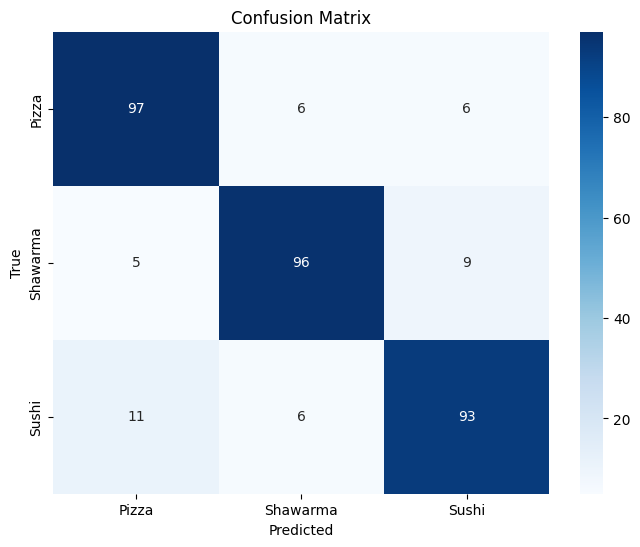
\includegraphics[width=0.45\textwidth]{model/neuralnetwork_confusion.png}
    \caption{Word Embedding Neural Network}
\end{table}

\subsection{Word Embedding - Linear and Logistic Regression}
We also evaluated linear regression and logistic regression models using sklearn's LinearRegression and LogisticRegression classes, applying the same feature set as the neural network. For linear regression, the target labels were represented as one-hot encoded vectors, while for logistic regression, the target labels were encoded as indices.

The linear regression model achieved a validation accuracy of approximately 86.6\%, slightly outperforming the logistic regression model, which achieved 84.8\%. We hypothesize that this difference arises because linear regression directly minimizes the loss function, whereas logistic regression relies on iterative solvers, which may introduce additional complexity. Additionally, logistic regression may be more prone to overfitting due to its higher model complexity.

For linear regression, we experimented with hyperparameters such as setting `fit\_intercept` to False and `positive` to True. Disabling `fit\_intercept` resulted in a slightly lower accuracy of 85\%, while changing the `positive` parameter had no impact on accuracy, maintaining the default performance.

For logistic regression, we tested various solvers, including 'lbfgs', 'liblinear', 'newton-cg', 'newton-cholesky', 'sag', and 'saga'. The validation accuracies for these solvers were 83.9\%, 84.8\%, 84.2\%, 83.9\%, 83.8\%, and 83.9\%, respectively. Among these, the 'liblinear' solver performed best, achieving 84.8\% accuracy with both 'l1' and 'l2' regularization. Other solvers were tested with the default 'l2' regularization.

Overall, the linear regression model demonstrated slightly better performance compared to both the neural network and logistic regression models, suggesting that the dataset's features may not require highly complex representations. Logistic regression tables are omitted here, as their results closely resemble those of linear regression but with marginally lower accuracy.

\begin{table}[h]
    \centering
    \begin{tabular}{lccc}
        \hline
        Category     & Precision                              & Recall & F1-score \\
        \hline
        Pizza        & 0.86                                   & 0.89   & 0.87     \\
        Shawarma     & 0.89                                   & 0.87   & 0.88     \\
        Sushi        & 0.86                                   & 0.85   & 0.85     \\
        \hline
        Accuracy     & \multicolumn{3}{c}{0.87 (329 samples)}                     \\
        Macro avg    & 0.87                                   & 0.87   & 0.87     \\
        Weighted avg & 0.87                                   & 0.87   & 0.87     \\
        \hline                                                                    \\
    \end{tabular}
    \begin{tabular}{ccc}
        \hline
        Loss   & Bias   & Variance \\
        \hline
        0.2515 & 0.2515 & 0.0088   \\
        \hline                     \\
    \end{tabular}
    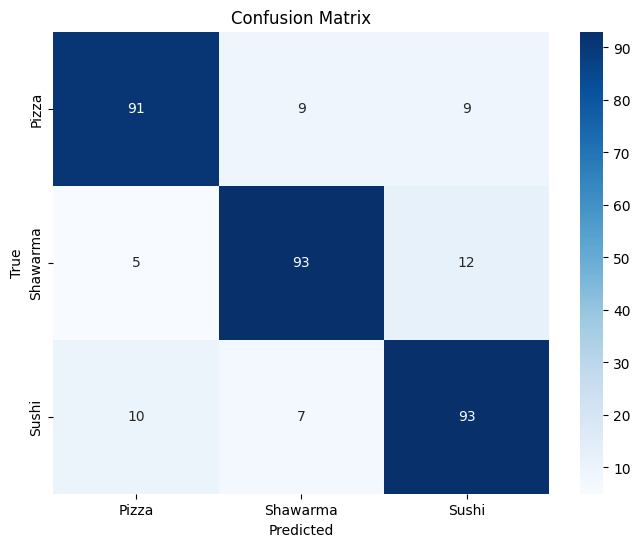
\includegraphics[width=0.45\textwidth]{model/linearregression_confusion.png}
    \caption{Word Embedding Linear Regression}
\end{table}

\subsection{Comparison of Word Embedding Models with Other Approaches}
The Word Embedding Neural Network yielded an accuracy of about 84.8\%, with a loss of 0.2269, a bias equal to its loss (0.2269), and a variance of 0.0731. The high bias suggests that it does not capture all complexity, while the variance stays relatively moderate. The Word Embedding Linear Regression achieved a slightly higher accuracy at 86.6\%, accompanied by a loss of 0.2515, bias of 0.2515, and a notably lower variance of 0.0088. Though its loss was higher, the overall bias-variance profile indicates more stable predictions compared to the neural network variant.

Compared to other models such as the MLPClassifier (90\% accuracy) and RandomForestClassifier (87\% accuracy), these word embedding approaches showed somewhat lower accuracies. The neural network had a higher variance component, while the linear regression model leaned toward higher bias. They both demonstrate that the selected text-based features might not require very deep representations, and simpler linear methods can yield competitive results. The neural network's and logistic regression's complexity may not be justified given the representation of the dataset, as indicated by the performance of the linear regression model.